% This file was created by matlab2tikz.
%
%The latest updates can be retrieved from
%  http://www.mathworks.com/matlabcentral/fileexchange/22022-matlab2tikz-matlab2tikz
%where you can also make suggestions and rate matlab2tikz.
%
\definecolor{mycolor1}{rgb}{0.00000,0.44700,0.74100}%
%
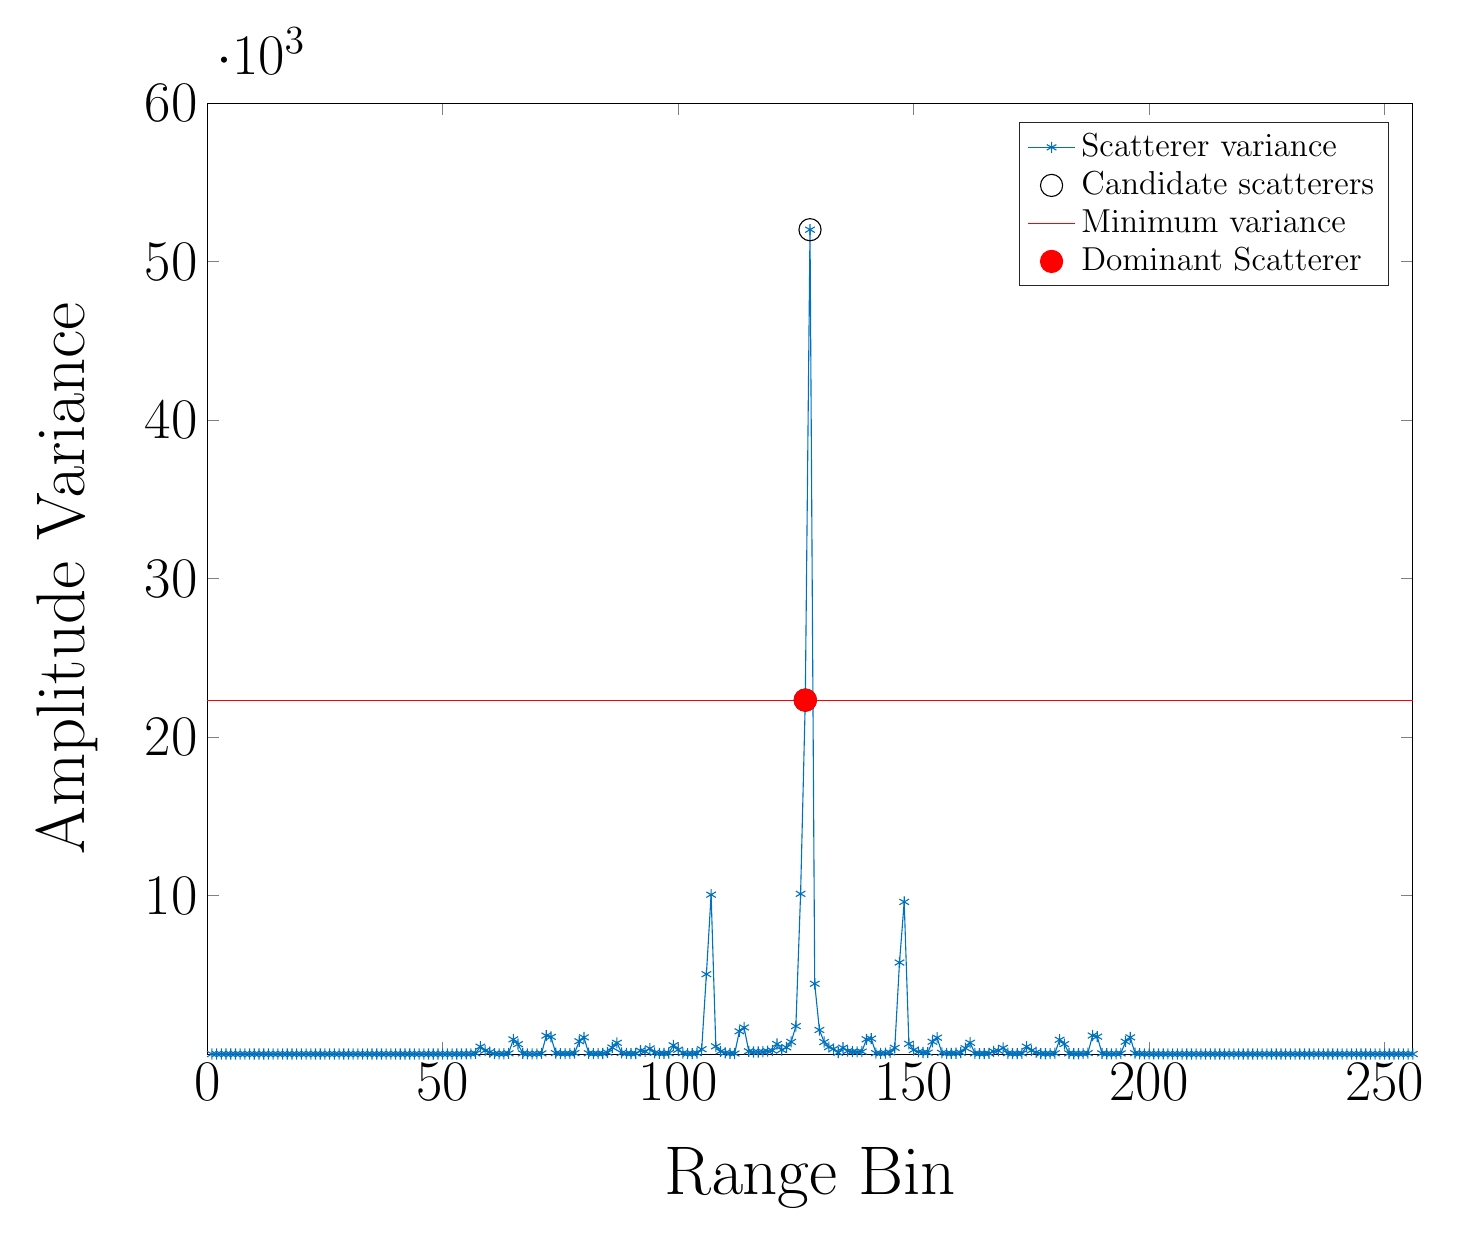
\begin{tikzpicture}

\begin{axis}[%
width=6.028in,
height=4.754in,
at={(1.011in,0.642in)},
scale only axis,
xmin=0,
xmax=256,
xlabel style={font=\fontsize{25}{20}\selectfont\color{black}, yshift = -10},
xlabel={Range Bin},
ymin=0,
ymax=60000,
ylabel style={font=\fontsize{25}{20}\selectfont\color{black}, yshift=10pt},
ylabel={Amplitude Variance},
axis background/.style={fill=white},
tick label style={font=\fontsize{20}{11}\selectfont\color{black}},
xtick distance = 50,
ytick distance= 1e4,
yticklabel={\ifdim\tick pt=0pt\else\pgfmathprintnumber{\tick}\fi}, 
scaled y ticks=base 10:-3,
legend style={legend cell align=left, align=left, draw=white!15!black, font=\fontsize{12}{11}\selectfont\color{black}}
]
\addplot [color=mycolor1, mark=asterisk, mark options={solid, mycolor1}]
  table[row sep=crcr]{%
1	1.9133938710127\\
2	2.01072279916104\\
3	1.90058203394593\\
4	1.88378981609597\\
5	1.8478207975461\\
6	1.98347699479647\\
7	1.89872916806568\\
8	2.03189519032328\\
9	1.90112975728777\\
10	1.99553746416861\\
11	2.01374019624089\\
12	2.09836204539017\\
13	2.06227827424652\\
14	2.12185823456891\\
15	2.03859918049033\\
16	1.845245661314\\
17	2.07270440638032\\
18	2.01524253699117\\
19	2.0946155593745\\
20	2.03171287688091\\
21	2.09126071499639\\
22	2.12998451928258\\
23	2.03378926311033\\
24	2.27347384225681\\
25	2.20193768710672\\
26	2.02862284736567\\
27	2.21275528819339\\
28	2.28233776318313\\
29	2.29938376177454\\
30	2.36477223889563\\
31	2.35258179963599\\
32	2.30429158369687\\
33	2.35206064405741\\
34	2.35396837623126\\
35	2.41452565723408\\
36	2.41191386124048\\
37	2.42026157639091\\
38	2.62413472857586\\
39	2.56850577159116\\
40	2.7946491472182\\
41	2.6732532485586\\
42	2.76041694086011\\
43	3.00609946037035\\
44	3.18145501265013\\
45	3.21020407897488\\
46	3.3340302767689\\
47	3.54600972364066\\
48	3.50260219857389\\
49	3.8766086418855\\
50	4.19441994998233\\
51	4.4412405727336\\
52	5.06053174897812\\
53	5.40929588964922\\
54	6.5415279965314\\
55	9.14507844442924\\
56	15.0519461424467\\
57	39.9147620601247\\
58	467.555867660639\\
59	213.055564504016\\
60	120.565987442262\\
61	23.5718626160254\\
62	15.6267439669318\\
63	18.7429164340291\\
64	46.0204225796209\\
65	924.630081299313\\
66	624.3791768422\\
67	44.835406841558\\
68	15.3314608898529\\
69	11.0121316087715\\
70	14.6402359597468\\
71	40.3845778003644\\
72	1164.09800572068\\
73	1083.04946223052\\
74	61.9421232638481\\
75	30.8218200734104\\
76	26.4822330997694\\
77	32.4934070180211\\
78	60.8045501780425\\
79	807.964378162526\\
80	1052.93803156586\\
81	50.7639952163396\\
82	24.9614931399461\\
83	25.3665089785796\\
84	34.6822763542242\\
85	90.0302388764038\\
86	412.616432925964\\
87	709.521197682858\\
88	70.4704627923113\\
89	37.7515979202163\\
90	28.909715258636\\
91	32.7161513779526\\
92	213.995963367863\\
93	167.17466855772\\
94	352.750811963452\\
95	74.5612361698514\\
96	46.6921514192879\\
97	40.7292592015906\\
98	53.7753783289214\\
99	553.334724747479\\
100	272.745825837723\\
101	62.9702337993028\\
102	23.6562353616831\\
103	28.6386488078339\\
104	61.2646037443697\\
105	304.544103144069\\
106	5040.58819343192\\
107	10058.0935558378\\
108	486.270143992054\\
109	170.483535882326\\
110	77.7995851300929\\
111	42.1083765818408\\
112	34.3500883096186\\
113	1434.22091686599\\
114	1676.56860212765\\
115	172.914575371846\\
116	128.776437906702\\
117	129.978754750311\\
118	146.578983651699\\
119	181.035216301624\\
120	219.314394090354\\
121	634.630971049835\\
122	257.430724866297\\
123	421.054403103927\\
124	764.792884049211\\
125	1761.90288790021\\
126	10109.7199969574\\
127	22334.9321747989\\
128	52020.5564987292\\
129	4434.86746154475\\
130	1518.69413082832\\
131	759.196729938088\\
132	438.0368572698\\
133	326.523224926599\\
134	85.0656652066872\\
135	402.127154859699\\
136	187.316390913439\\
137	151.091735157512\\
138	138.515622479074\\
139	153.523359476704\\
140	931.876021703375\\
141	975.805936191809\\
142	59.3884464659696\\
143	48.2931581680193\\
144	62.1061653540574\\
145	102.953642132513\\
146	392.659099155085\\
147	5774.47944807882\\
148	9599.34787354486\\
149	647.706979933297\\
150	252.189930592577\\
151	142.584663834502\\
152	97.9649883304548\\
153	87.1012140646438\\
154	775.731748358594\\
155	1033.87137971855\\
156	74.8302638798941\\
157	47.324611827748\\
158	44.1542444330301\\
159	52.8498245801726\\
160	86.4869278695037\\
161	368.873145231315\\
162	712.003460485302\\
163	43.6867962734471\\
164	28.3921536341544\\
165	30.9206672758996\\
166	41.7469115041917\\
167	168.710784335025\\
168	206.586661871223\\
169	392.726507342833\\
170	52.9343450967726\\
171	27.0736242705292\\
172	23.4418308675402\\
173	44.7178399190357\\
174	473.405425090333\\
175	220.754276926185\\
176	111.989135912725\\
177	27.3791278506749\\
178	20.1353224521916\\
179	21.8887907736741\\
180	49.2998953783466\\
181	901.90304645969\\
182	628.408400634152\\
183	44.1234430768824\\
184	20.669674341607\\
185	17.716028790995\\
186	24.4548947124522\\
187	58.5183771065465\\
188	1168.76912884724\\
189	1101.25976889245\\
190	44.365095390368\\
191	17.8942269004586\\
192	14.4401480055255\\
193	18.2876278489029\\
194	39.8088557316537\\
195	779.678167552672\\
196	1052.28402448725\\
197	54.1173029789816\\
198	20.8858804842876\\
199	12.4580109915738\\
200	9.43720634815922\\
201	7.45820324957887\\
202	6.7409856328254\\
203	6.24786378954438\\
204	5.78374877049891\\
205	5.22341441451239\\
206	5.36648882210141\\
207	5.08768963190121\\
208	4.7541276152746\\
209	4.54650366302474\\
210	4.34928636340311\\
211	4.27544104616072\\
212	3.96149868708858\\
213	3.79984734386163\\
214	3.75335376397874\\
215	3.55382808024156\\
216	3.33906780783109\\
217	3.2182660095367\\
218	3.083163957648\\
219	2.99906362788988\\
220	2.87185963531737\\
221	2.85588003683741\\
222	2.70608576513909\\
223	2.92929818451152\\
224	2.79802652959837\\
225	2.61584594152127\\
226	2.56609915258513\\
227	2.48602160283973\\
228	2.52296739363419\\
229	2.47179727610708\\
230	2.42983196707561\\
231	2.33309469061028\\
232	2.3201545764392\\
233	2.36510361966071\\
234	2.29592941574246\\
235	2.06841894427994\\
236	2.20352276065941\\
237	2.18560663998336\\
238	2.14855993431592\\
239	2.15290004936119\\
240	2.12088813629976\\
241	2.06865221157781\\
242	2.14894753386742\\
243	2.07351400343677\\
244	2.07905497313625\\
245	2.04323682660534\\
246	2.15851964442678\\
247	1.93360921061516\\
248	2.0024913022139\\
249	2.05876418202431\\
250	2.03315703674219\\
251	2.0884965340862\\
252	1.92358563275556\\
253	1.96525319547271\\
254	2.0880168262253\\
255	1.9932171662393\\
256	1.90410475031383\\
};
\addlegendentry{Scatterer variance}

\addplot [color=black, only marks, mark size=4.0pt, mark=o, mark options={solid, black}]
  table[row sep=crcr]{%
127	22334.9321747989\\
128	52020.5564987292\\
};
\addlegendentry{Candidate scatterers}

\addplot [color=red]
  table[row sep=crcr]{%
0	22334.9321747989\\
300	22334.9321747989\\
};
\addlegendentry{Minimum variance}

\addplot [color=red, only marks, mark size=4.0pt, mark=*, mark options={solid, fill=red, red}]
  table[row sep=crcr]{%
127	22334.9321747989\\
};
\addlegendentry{Dominant Scatterer}

\end{axis}
\end{tikzpicture}%